\section{VPN в контейнере}

Технология VPN\footnote{VPN (англ. Virtual Private Network) "--- обобщенное название технологий, позволяющих обеспечить одно или несколько сетевых соединений поверх другой сети (например, Интернет)} позволяет устанавливать безопасное сетевое соединение между компьютерами.
Для того чтобы VPN работала в контейнере, необходимо разрешить использование TUN/TAP устройств для контейнера.
\begin{figure}[ht]
    \centering
	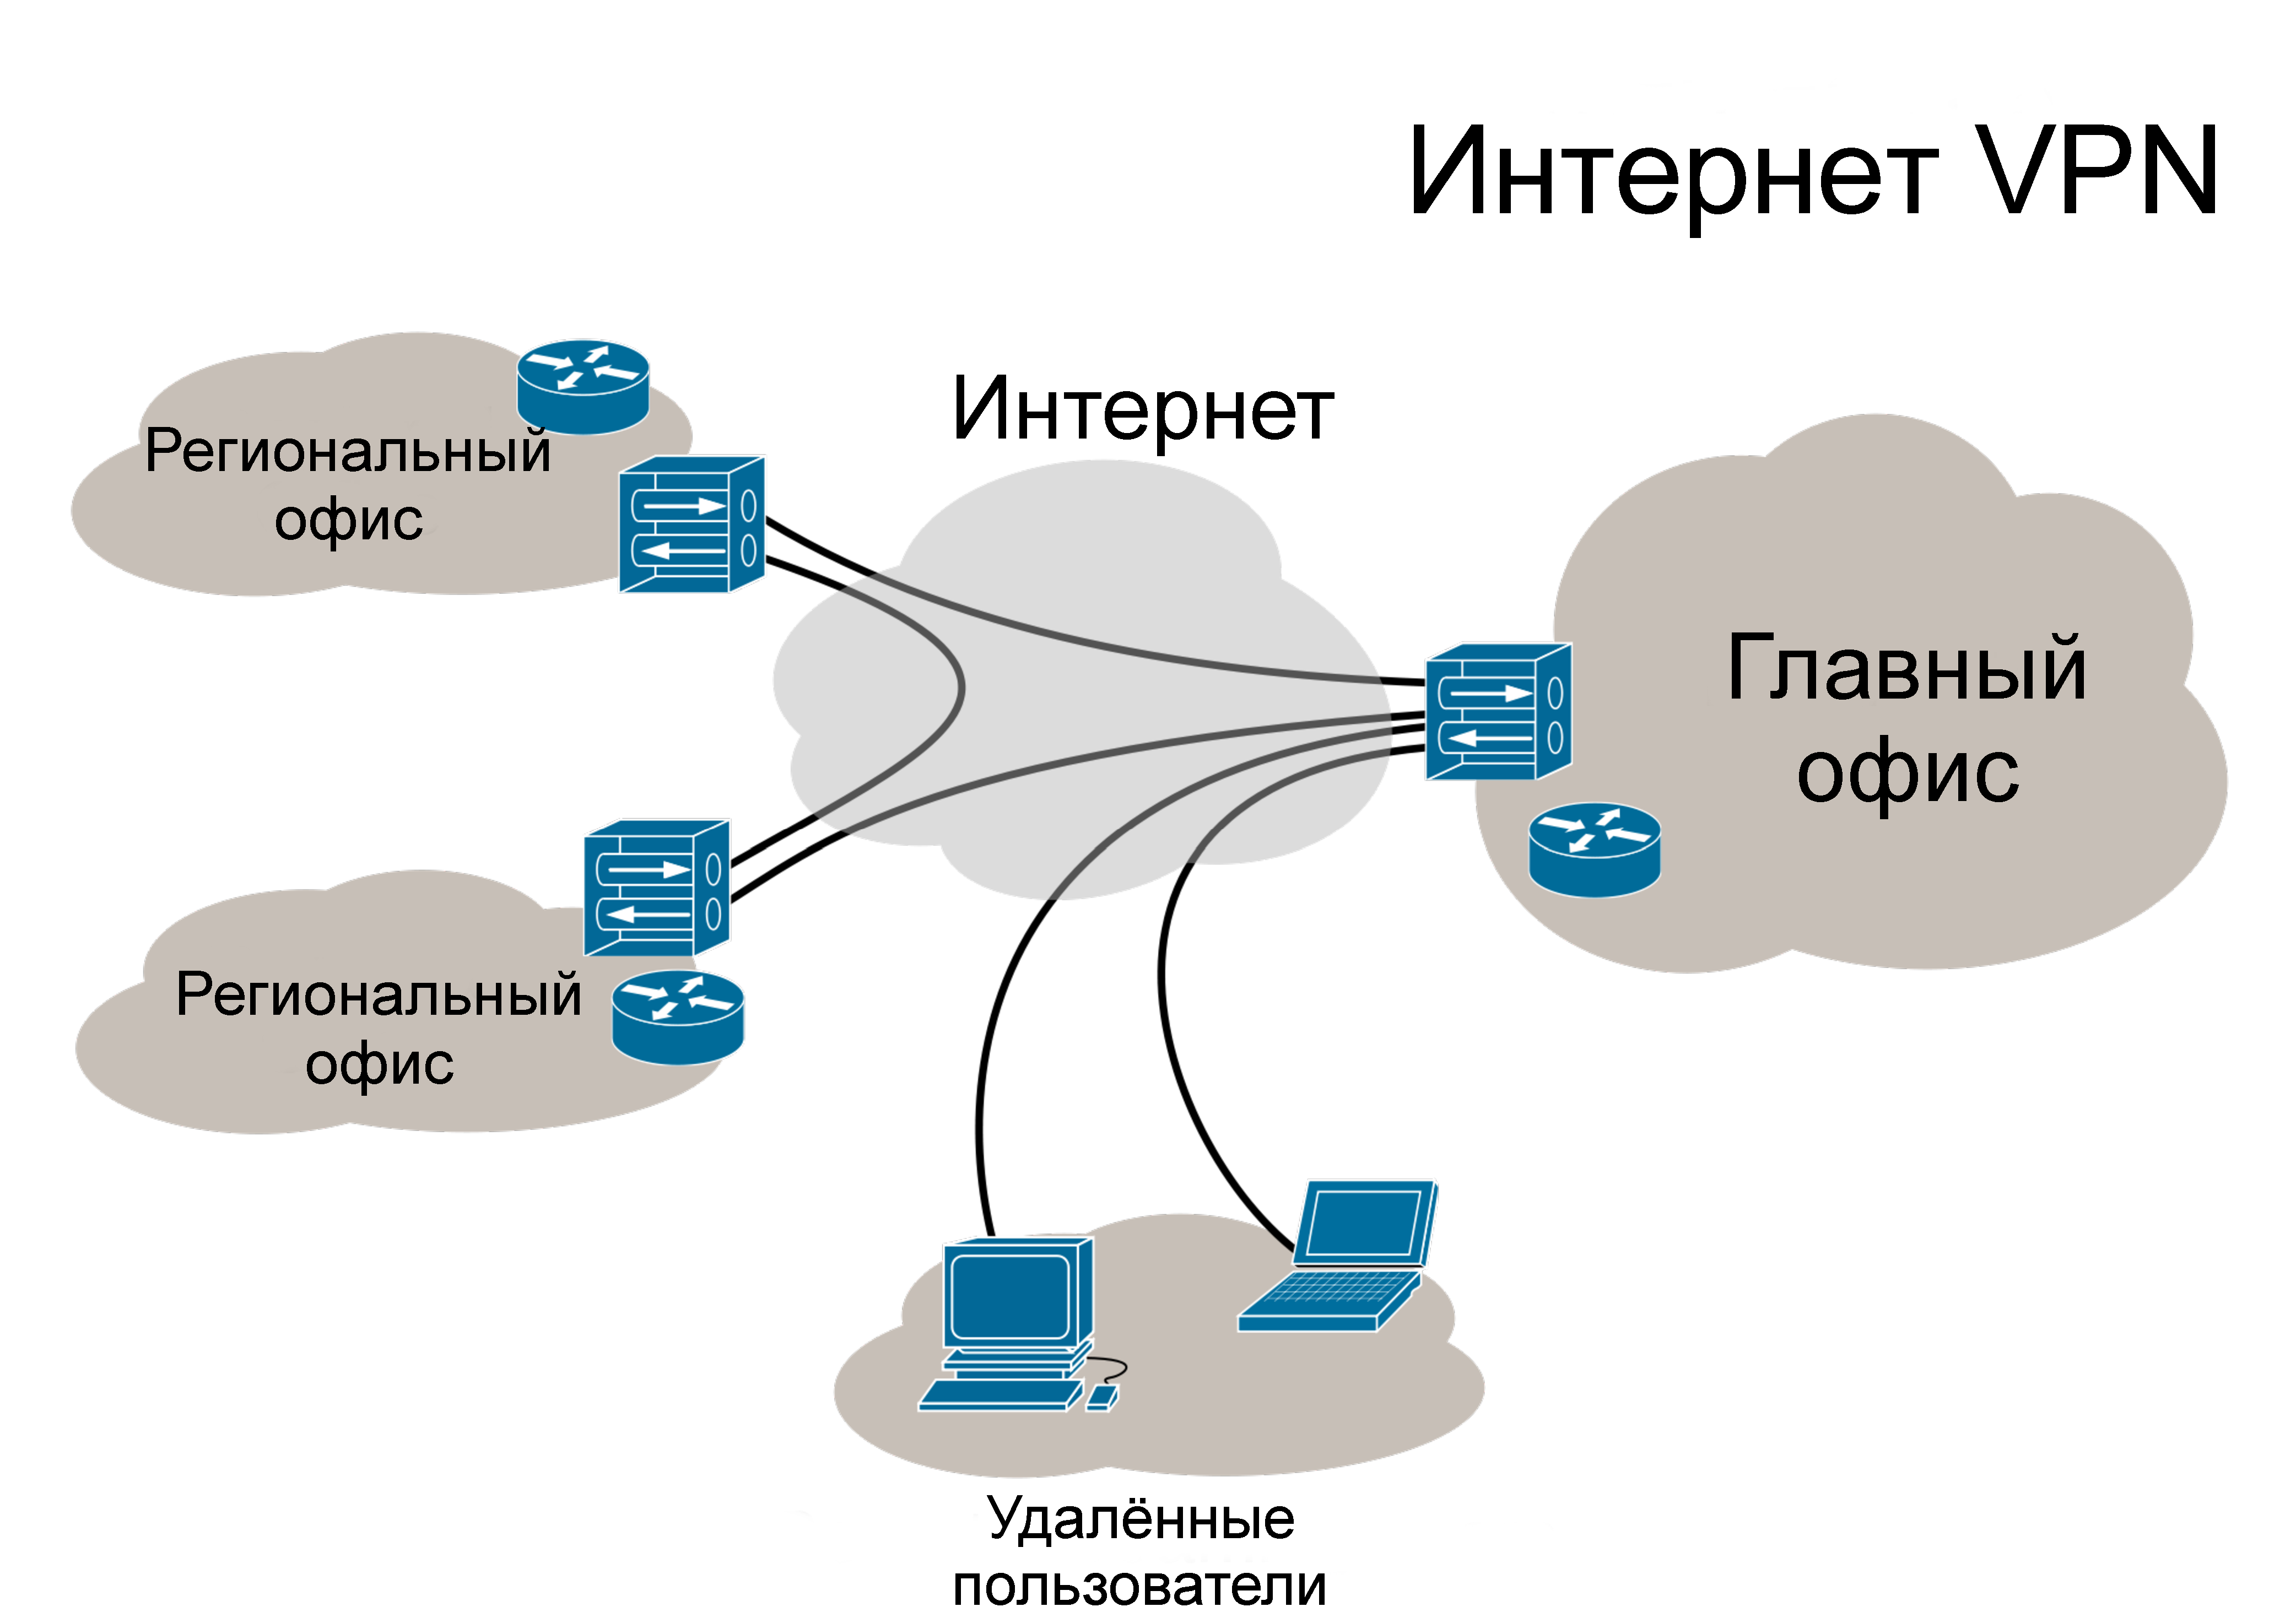
\includegraphics[width=\linewidth]{vpn.pdf}
	\caption{Схема работы VPN}\label{pic:vpn}
\end{figure}

Прежде чем запускать контейнер нужно убедиться, что модуль TUN загружен:
\begin{lstlisting}
# lsmod | grep tun
\end{lstlisting}

В случае, если он не загружен, загрузить его можно следующей командой:
\begin{lstlisting}
# modprobe tun
\end{lstlisting}
\begin{lstlisting}
# lsmod | grep tun
tun     1957    0
\end{lstlisting}

Разрешаем использовать устройство TUN контейнеру:
\begin{lstlisting}
# vzctl set 101 --devnodes net/tun:rw --save
CT configuration saved to /etc/vz/conf/101.conf
\end{lstlisting}
\begin{lstlisting}
# vzctl set 101 --devices c:10:200:rw --save
CT configuration saved to /etc/vz/conf/101.conf
\end{lstlisting}
\begin{lstlisting}
# vzctl set 101 --capability net_admin:on --save
CT configuration saved to /etc/vz/conf/101.conf
\end{lstlisting}

Запускаем контейнер:
\begin{lstlisting}
# vzctl start 101
Starting container...
Opening delta /vz/private/101/root.hdd/root.hdd
Adding delta dev=/dev/ploop17343 img=/vz/private/101/root.hdd/root.hdd (rw)
Mounting /dev/ploop17343p1 at /vz/root/101 fstype=ext4 data='balloon_ino=12,' 
Container is mounted
Adding IP address(es): 192.168.0.101
Setting CPU units: 1000
Setting devices
Container start in progress...
\end{lstlisting}

Создаем в контейнере собственное устройство TUN:
\begin{lstlisting}
# vzctl exec 101 mkdir -p /dev/net
# vzctl exec 101 mknod /dev/net/tun c 10 200
# vzctl exec 101 chmod 600 /dev/net/tun
\end{lstlisting}

На этом настройка устройства TUN окончена.
Далее необходимо установить ПО для работы с VPN.
Например одну из программ:
\begin{itemize}
    \item tinc (\url{http://tinc-vpn.org});
    \item OpenVPN (\url{http://openvpn.net});
    \item VTun (\url{http://vtun.sourceforge.net}).
\end{itemize}

Для установки сервера OpenVPN, можно обратиться к официальной документации, расположенной по адресу: \url{http://openvpn.net/index.php/open-source/documentation.html}

\clearpage
